\chapter{Implementazione dei comportamenti e delle strategie}
\label{implementation:intro}

In questo capitolo verranno analizzate le strategie di scelta della coda da parte del cliente. In particolare queste strategie determinano la coda che il cliente deciderà di seguire durante la \textit{fase di scelta della coda} e durante la \textit{fase di attesa in coda e jockeying}. 

Come introdotto all'inizio della relazione, obiettivo di questo progetto è analizzare le varie configurazioni di casse all'interno del supermercato, al variare del tipo di casse, della quantità di clienti presenti nel negozio e alla strategia di scelta della coda dei clienti, pertanto è necessario disporre di strategie che sfruttano calcoli basati su variabili diverse: le variabili in gioco saranno il numero di elementi nel carrello, il numero di persone e il tempo medio di attesa.

Se un cliente entra nel supermercato con l'intenzione di usare le casse self-scan, chiaramente non sarà dotato di strategie di scelta della coda e di jockeying, dal momento che le casse self-scan hanno sempre un'unica coda condivisa. Anche nel caso in cui le casse standard abbiano un'unica coda condivisa, come capita in molti negozi, il cliente non avrà una strategia di scelta della coda o di jockeying. Al contrario invece, dopo la fase di shopping il cliente dovrà scegliere la coda tra le code disponibili delle casse standard e delle casse self-service; una volta che esso si accoda in una cassa standard, può decidere di cambiare coda e quindi effettuare il jockeying, se ritiene, con la propria strategia, che nelle casse a lui più vicine ci sia un tempo minore di attesa.

Lo scopo del progetto è indagare sulla configurazione di casse migliori, quindi ad ogni simulazione tutti i clienti avranno la stessa strategia di scelta della coda e di jockeying per creare una netta distinzione tra simulazioni diverse.

\section{Fase di scelta della coda}
\label{implementation:queuechoice}

Alla fine della \textit{fase di shopping}, il cliente che non vuole andare alla cassa self-scan, deve scegliere quale coda seguire tra quelle disponibili, ovvero tra le code associate a casse aperte. 

Una strategia è una scelta della coda $q$ che minimizza una certa funzione $f(q)$, come riportato nel capitolo precedente alla \ref{eq:strategy}. 

Al fine di definire le strategie, è importante notare che la funzione $\text{basket-size}(c_i)$ non deve essere deterministica, come già introdotto nel capitolo precedente: il cliente fa una stima del numero di elementi nel carrello degli altri elementi, non ne è però certo, per questo questa funzione ha una probabilità di errore che rende la stima più veritiera, e si può ridefinire:
\begin{equation}\label{eq:estimate-basket-size}
\text{estimate-basket-size}(c_i) = \text{basket-size}(c_i) + e_i
\end{equation}
dove $e_i$ è l'errore commesso nella stima e può essere sia positivo che negativo. L'errore dipende dalla grandezza del carrello, in particolare più elementi ci sono nel carrello più l'errore aumenta; intuitivamente in questo modello si è deciso di far variare l'errore in modo logaritmico rispetto alla grandezza del carrello, in base alla formula:
\begin{equation}\label{eq:error-basket-size}
e_i = \frac{\text{basket-size}(c_i)}{d}
\end{equation}
dove $d \in \mathbb{R}$, $d \ge 1$ e se $d = 1$ non viene commesso alcun errore sulla stima. 
La quantità estimate-basket-size diventa dunque una variabile aleatoria normale con media la basket-size reale e deviazione standard l'errore commesso sulla stima.

Le 4 strategie di scelta della coda prese in considerazione per il modello sono:

\begin{enumerate}
\item \textbf{Minimo numero di elementi}: viene scelta la coda con il minimo numero di elementi nei carrelli di tutte le persone in attesa. La funzione da minimizzare è quindi per una coda $q \in Q$ dove $Q$ è l'insieme di tutte le code disponibili:
\begin{equation}
f(q) = \sum\limits_{i=1}^N \text{estimate-basket-size-size}(c_i) 
\end{equation}
dove $c_i \in q$ è un cliente in coda, $\text{estimate-basket-size-size}(c_i)$ è il numero di elementi che ha nel suo carrello e $N = |q|$ è il numero di clienti in coda in $q$.
\item \textbf{Minimo numero di persone}: viene scelta la coda con il minimo numero di persone accodate. La funzione da minimizzare per $q \in Q$ è:
\begin{equation}
f(q) = |q|
\end{equation}
\item \textbf{Minimo tempo d'attesa in base al tempo di servizio medio}:
viene scelta la coda con il tempo d'attesa minimo, calcolato in base al tempo di servizio medio.
Il \textit{tempo di servizio totale di una coda} è calcolato come somma del tempo di servizio per ogni cliente della coda. Il tempo di servizio per un cliente comprende il \textbf{tempo di transazione} e il \textbf{tempo di pausa} tra un cliente e un altro, e variano a seconda del tipo di cassa, come illustrato nella sezione \ref{model:cashdesks}. Le formule per il calcolo dei tempi per la cassa standard \ref{eq:transaction-time-standard} e \ref{eq:break-time-standard}, comprendendo la stima della grandezza del carrello, diventano dunque:

\begin{equation}\label{eq:transaction-time-standard-estimate}
\text{transaction-time}_i = e^{a log(\text{estimate-basket-size}(c_i)) + b}
\end{equation}
\begin{equation}\label{eq:break-time-standard-estimate}
\text{break-time}_i = \frac{\beta^{\alpha} \text{estimate-basket-size}(c_i)^{\alpha - 1} e^{- \beta \text{estimate-basket-size}(c_i)}}{\Gamma (\alpha)}
\end{equation}

e per la cassa self-service, le \ref{eq:transaction-time-self-service} e \ref{eq:break-time-self-service} diventano:

\begin{equation}\label{eq:transaction-time-self-service-estimate}
\text{transaction-time}_i = e^{a log(\text{estimate-basket-size}(c_i)) + b}
\end{equation}
\begin{equation}\label{eq:break-time-self-service-estimate}
\text{break-time}_i = e^{c log(\text{estimate-basket-size}(c_i)) + d}
\end{equation}

I tempi di servizio per ogni cliente di una coda sono quindi sommati per calcolare il tempo servizio totale per quella coda. Il tempo di servizio totale di una coda $q_j$, $j = 1,\ldots ,M$, dove $M$ è il numero totale di code del supermercato, è pertanto:
\begin{equation}\label{eq:total-service-time}
\text{total-service-time}(q_j) = \sum\limits_{i=1}^N \left( \text{transaction-time}_i + \text{break-time}_i \right)
\end{equation}
Il tempo di servizio medio per le code è la somma dei tempi totali di servizio divisa per il numero di code. Viene scelta la coda con il tempo totale minimo, mettendo insieme le \ref{eq:transaction-time-standard-estimate}, \ref{eq:break-time-standard-estimate}, \ref{eq:transaction-time-self-service-estimate}, \ref{eq:break-time-self-service-estimate} e \ref{eq:total-service-time} si ottiene la funzione da minimizzare:
\begin{equation}
f(q) = |q| * \frac{1}{M}\sum\limits_{j=1}^M \left( \text{total-service-time}(q_j) \right)
\end{equation}
\item \textbf{Minimo tempo d'attesa in base alla \textit{power regression}}: viene scelta la coda con il tempo d'attesa minimo, calcolato in base al tempo di transazione e il tempo di pausa medi per quella coda. Il tempo di servizio totale per una coda è calcolato anche qui in base alla \ref{eq:total-service-time}. La funzione da minimizzare è:
\begin{equation}
f(q) = |q| * \text{total-service-time}(q)
\end{equation}
\end{enumerate}

\section{Fase di attesa in coda e jockeying}

Quando il cliente è nella \textit{fase di attesa in coda} ha la possibilità di cambiare la propria scelta se nota che nelle code adiacenti il tempo di attesa è minore che nella propria; le code adiacenti implicate nel calcolo sono quelle che hanno distanza minore o uguale del \textbf{parametro di adiacenza}, descritto nel capitolo precedente, rispetto a dove il cliente è già accodato. Una coda è distante 1 da un'altra coda se fisicamente nella griglia della simulazione esse compaiono una di fianco all'altra. Nella pratica la coda in cui il cliente è presente in un determinato momento svolge la funzione di coda pivot e le altre code prese in considerazione per fare jockeying sono quelle adiacenti alla coda pivot.

Le strategie seguite nel jockeying sono due, e coincidono con le prime due strategie di scelta della coda, descritte nella sezione precedente. Anche in questo caso il cliente stima le grandezze dei carrelli degli altri clienti in base alle \ref{eq:estimate-basket-size} e \ref{eq:error-basket-size}.
Entrambe le strategie necessitano di un \textbf{threshold}, che è un parametro del modello; dopo aver trovato la coda adiacente con tempo di attesa minore, viene calcolato un "guadagno" di fare jockeying, e se questo guadagno è più alto del threshold, allora il cliente cambia coda, altrimenti no; questo parametro serve a simulare il fatto che le persone in coda tendono sempre a preferire la propria posizione corrente, e a cambiare coda solo quando conviene tanto. 
Inoltre abbiamo pensato che non tutte le persone al supermercato vogliono fare jockeying, ci sono alcuni che neanche lo considerano e non guardano le casse adiacenti per valutarne il tempo medio d'attesa, pertanto abbiamo impostato un parametro che rappresenta la probabilità di fare jockeying, in modo che prima di scegliere si estragga un numero casuale e si decida.

\begin{enumerate}
\item \textbf{Minimo numero di elementi}: viene scelta la coda con il minimo numero di elementi nei carrelli di tutte le persone in attesa. Il "guadagno" nel cambiare coda è calcolato come:
\begin{equation}
	g = \# \text{elementi nei carrelli} - \min\limits_{q \in Q_{\text{adj}}} \# \text{elementi nei carrelli}
\end{equation}
dove $Q_{\text{adj}}$ è l'insieme delle code adiacenti alla coda corrente. Se questo valore è più alto del threshold, significa che il guadagno è abbastanza alto e il cliente cambia coda.
\item \textbf{Minimo numero di persone}: viene scelta la coda con il minimo numero di persone accodate. Il "guadagno" nel cambiare coda è calcolato come:
\begin{equation}
	g = i - \min\limits_{q \in Q_{\text{adj}}} |q|
\end{equation}
dove $0 < i \le |q_{\text{current}}|$ è la posizione del cliente nella coda corrente.
\end{enumerate}

Nella figura \ref{fig:jockeying-flowchart} è riportato il grafico che rappresenta il comportamento del cliente in fase di jockeying.

\begin{figure}[htp!]
	\centering
	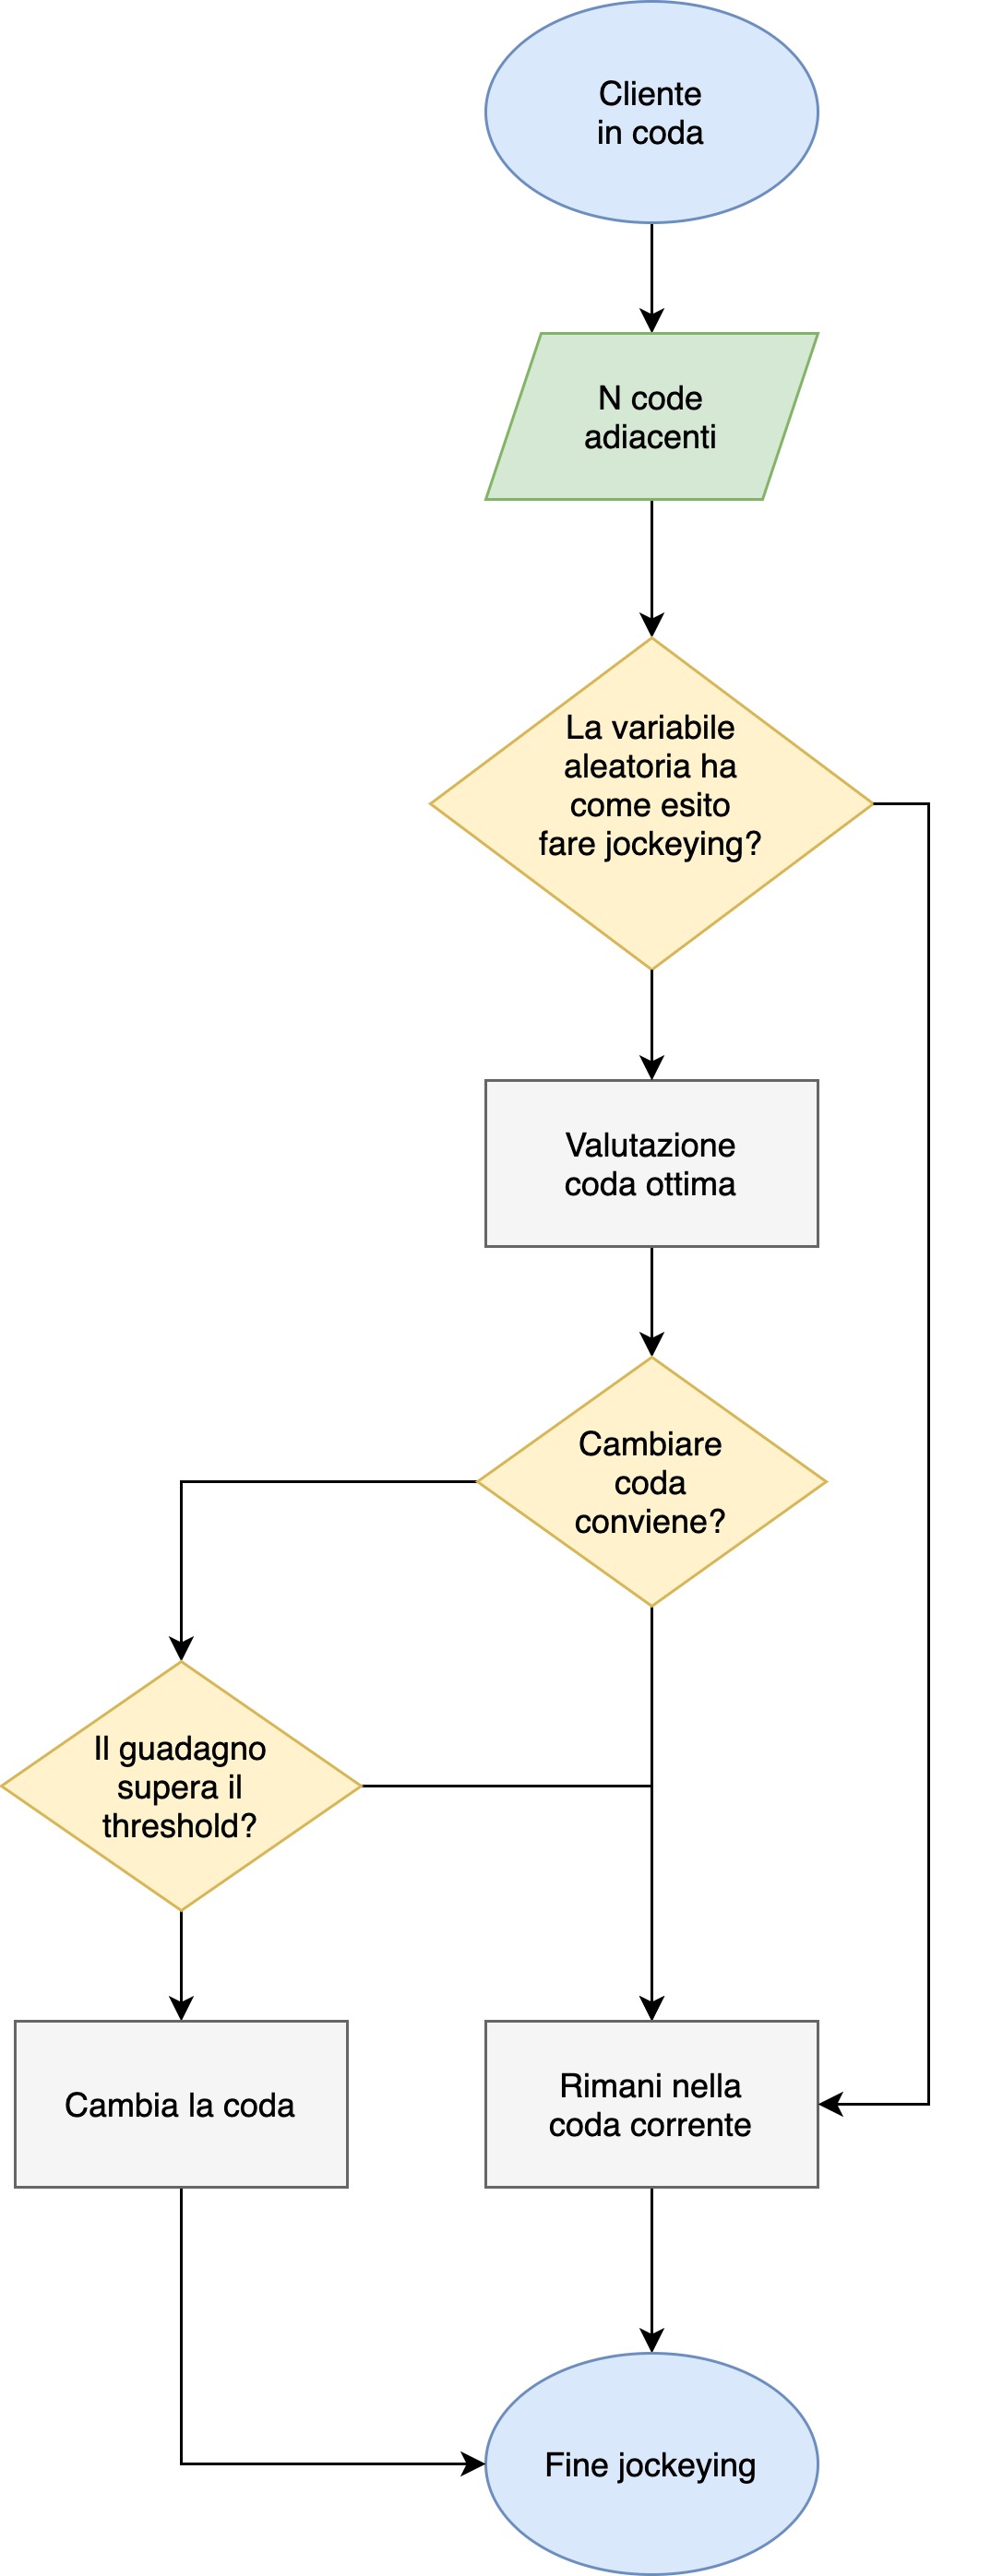
\includegraphics[width=6cm]{"images/jockeying-flowchart.png"}
	\caption{Workflow jockeying.}
	\label{fig:jockeying-flowchart}
\end{figure}

In questo capitolo sono state descritte le strategie utilizzate nelle fasi di scelta della coda e di jockeying da parte del cliente; le strategie di scelta della coda come si è visto sono 4 e sono state descritte in ordine di complessità; le strategie per fare jockeying sono invece 2 e si basano solamente sul numero di elementi nel carrello e sul numero di clienti in coda. Probabilmente non tutte le strategie sono realistiche e utilizzate concretamente dalle persone in coda al supermercato, l'obiettivo non è indagare sulla scelta effettuata dagli umani in coda, ma capire quale sia la strategia migliore che può essere implementata in un vero supermercato ad esempio con un display che suggerisce quale sia la coda migliore in un dato istante. Nel prossimo capitolo finalmente vedremo i risultati del nostro modello, in particolare metteremo a confronto la nostra simulazione con quella dell'articolo \cite{article1} allo scopo di calibrare e validare il modello; introdurremo quindi man mano le espansioni che abbiamo apportato, lo scopo rimarrà sempre quello di diminuire i tempi d'attesa dei clienti e migliorare la loro esperienza.
